Our robot Dora is essentially a Pioneer 3D-X differential robot platform with an in-house central supporting construction attached to it. This construction serves as support for the various sensors and the laptop which is the brain of the robot (see Fig~\ref{fig:dora}). In terms of sensing Dora is equipped with 2 laser rangefinders and 1 depth camera. These sensors are primarily used to ensure safe navigation 
and people detection. This year, we are going to significantly improve Dora's hardware itself as well as how the software handles this hardware. This will provide more support for:

\begin{itemize}
\item \textit{Human-Robot-Interaction (HRI)} - Last year, speech understanding and reproduction were strongly limited due to the use of the laptop's build-in audio equipment. We are going to extend audio recording and reproduction capabilities by mounting a microphone and a speaker. Additionally, we are going to improve Dora's appearance to be more user-friendly which in turn will improve HRI. 
\item \textit{Safe and robust navigation} - We are investigating usage of Pioneer's sonar to detect small objects very close to the ground level. Moreover, Pioneer's bumpers will be used to stop the robot when an object is hit. 
\item \textit{Object recognition} - another depth camera with short range will be added to allow detection and recognition of small household objects.
\end{itemize}
 
\begin{figure}[!htb]
\centering
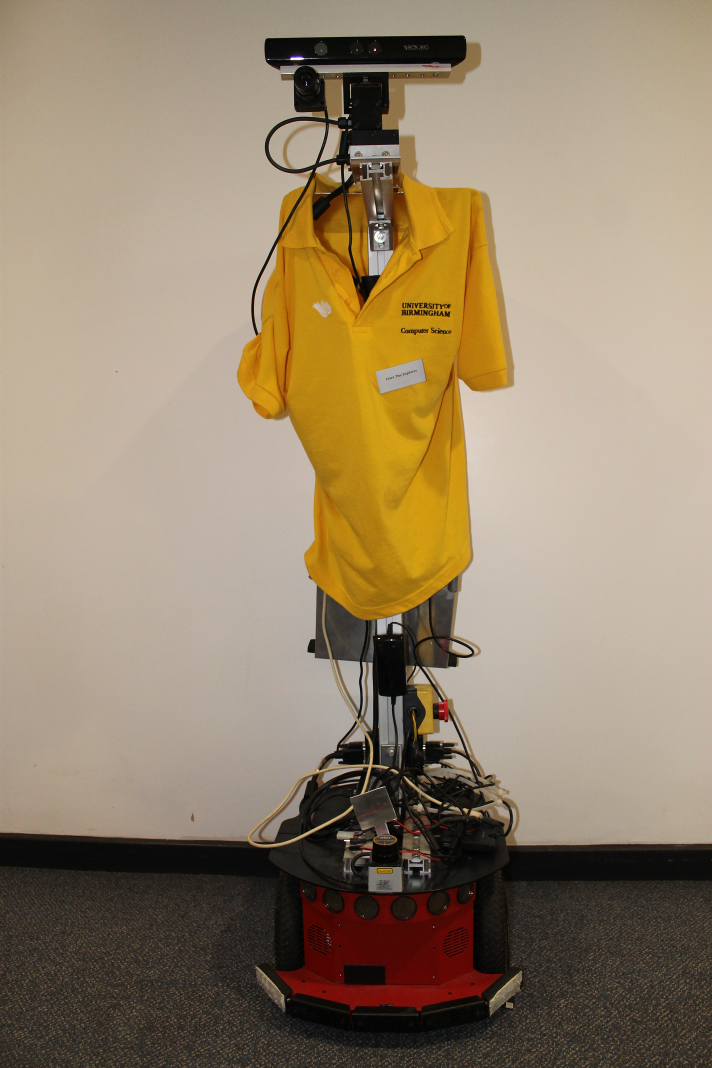
\includegraphics[width=2.in]{dora_new.png}
\caption{Dora is an extended Pioneer 3D-X robot with sensors such as laser range finders, depth cameras and a laptop mounted on top.}
\label{fig:dora}
\end{figure}  


